\chapter{Raspberry PI}
Mit dem Raspberry PI bietet die Raspberry PI Foundation einen Einplatinencomputer bereit, der für Experimente und Entwicklung von Programmen geeignet ist. Sein günstiger Preis von weniger als 40 Dollar und die Größe einer Kreditkarte tragen zu seinem Erfolg bei. Weiterhin existieren verschiedene Varianten des Computers, welche sich hauptsächlich in der Rechenleistung unterscheiden. Ursprünglich sollte der Raspberry PI zum Experimentieren von Studenten verwendet werden, fand jedoch schnell Anklag in divseren anderen Bereichen außerhalb von Universitäten.\\ %https://www.raspberrypi.org/about/
Für diese Arbeit wurde ein Raspberry PI 2 vorgeschrieben, da er eine kostengünstige Alternative darstellt, um hardwarenahe Software zu verwirklichen. Hierbei tragen besonders die General Purpose Input/Output Pins eine wichtige Rolle. Weiterhin verfügt der Raspberry PI über eine Ethernet Schnittstelle, welche zur Kommunikation dient. Da es sich um einen Einplatinencomputer und nicht um einen klassischen Mikrocontroller handelt, findet sich auf dem Raspberry PI ein Betriebssystems wieder, welches eine Erleichterung für die Softwareentwicklung darstellt. Hierzu zählt insbesondere die Umsetzung des TCPI/IP Stacks.\\ % Quellen?

\section{Betriebssystem}
Die Betriebssysteme für den Raspberry PI sind zahlreich. Am häufigsten ist jedoch eine Linux-Distribution anzutreffen. In diesem Projekt kommt Raspbian, ein auf Debian angepasstes Betriebssystem. Die Installation von Raspbian findet mit dem NOOBS-Installer, ein von der Raspberry PI Foundation bereitgestellter Installationsassistent, statt. % https://www.raspberrypi.org/help/noobs-setup/
Das Betriebssystem vereinfacht die Softwareentwicklung dahingehend, dass es verschiedene Schnittstellen für den Zugriff auf die Hardware anbietet. Die für dieses Projekt am wichtigsten Schnittstellen sind einerseits die GPIO Pins und andererseits der Zugriff auf das Ethernet.

\section{GPIO}
Von den insgesamt 40 Pins sind 26 GPIO Pins. Bei den anderen handelt es sich Pins für die Stromversorgung. Abbildung \ref{gpio-pins} zeigt die Belegung der Pins des Raspberry PI 2.
\begin{figure}[ht]
	\centering
	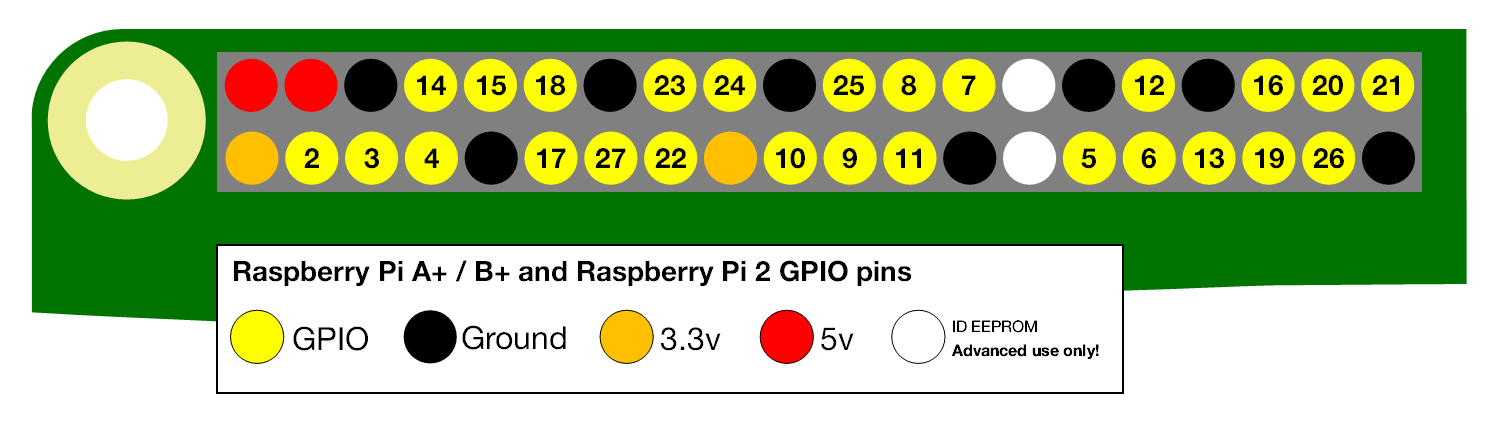
\includegraphics[width=0.7\textwidth]{bilder/gpio-pins.png}
	\caption{Pin Belegung Raspberry PI 2}
	\label{gpio-pins}
\end{figure}

\section{Netzwerk}
